\documentclass[11pt,a4paper]{article}

\usepackage[sc]{mathpazo}\linespread{1.04}
\usepackage[margin=2.4cm]{geometry}
\usepackage{amsmath,amssymb,amsthm,mathtools}
\usepackage{booktabs,array,multirow}
\usepackage{graphicx}
\usepackage{algorithm}
\usepackage[noend]{algpseudocode}
\usepackage{listings}
\usepackage{xcolor}
\usepackage{caption}
\usepackage[hidelinks]{hyperref}
\usepackage{cleveref}
\usepackage[section]{placeins}

\definecolor{codebg}{HTML}{F6F6F4}
\lstset{basicstyle=\ttfamily\footnotesize, backgroundcolor=\color{codebg},
  frame=single, rulecolor=\color{black!15}, columns=fullflexible, keepspaces=true,
  breaklines=true, showstringspaces=false, language=Python,
  keywordstyle=\color{black}\bfseries, commentstyle=\color{black!55}\itshape}
\captionsetup{font=small,labelfont=bf}

\newtheorem{lemma}{Lemma}
\newtheorem{theorem}{Theorem}
\newtheorem{proposition}{Proposition}
\theoremstyle{remark}
\newtheorem{remark}{Remark}

\newcommand{\R}{\mathbb{R}}
\newcommand{\eps}{\varepsilon}
\newcommand{\Th}{\Theta}
\newcommand{\Oh}{\mathcal{O}}
\renewcommand{\Re}{\operatorname{Re}}

\title{A Fast Transform for Evaluating Internal Potential-Field Models\\
(IGRF / CHAOS type) at Scattered Points in 3-D}
\author{Algorithm description, analysis and benchmarks\\[2pt]
\small reference implementation: \texttt{fastpot} (Python, FINUFFT)}
\date{8 October 2026}

\newcommand\SPEEDUPDOUBLE{$103\times$}
\newcommand\SPEEDUPDOUBLETEN{$46\times$}
\newcommand\SPEEDUPSINGLE{$122\times$}

\begin{document}
\maketitle

\begin{abstract}
Internal geomagnetic field models such as the IGRF and the CHAOS series are expressed as
solid spherical harmonic expansions of a scalar potential. Evaluating such a model of maximum
degree $L$ at $M$ arbitrary points $(r_i,\theta_i,\varphi_i)$ costs $\Oh(ML^2)$ by direct
summation. We show that, after the change of variables $u=a/r=u_c+u_d\cos\psi$, every
component of the field $\mathbf B=-\nabla V$ (and $V$ itself) is \emph{exactly} a
band-limited trivariate Fourier series in $(\psi,\theta,\varphi)$, of degree $\le L+2$ in
$\psi$, $\le L$ in $\theta$ and $\le L$ in $\varphi$. Evaluation at scattered points is
therefore a single three-dimensional type-2 non-uniform FFT (NUFFT). The resulting algorithm
needs a one-off $\Oh(KL^3)$ precomputation and then $\Oh(KL^2\log L + M w^3)$ work, where
$K\le L+2$ is the radial degree (typically $4$--$16$ for satellite data) and
$w\approx\log_{10}(1/\eps)+1$ is the NUFFT kernel width. Apart from the user-selected
tolerance $\eps$ the method makes no approximation: no quadrature grid, no interpolation in
radius, and no special treatment of the poles. Against an optimised, multithreaded direct
evaluator, the method is about $100\times$ faster in double precision at $\eps=10^{-6}$
($45\times$ at $\eps=10^{-10}$, $120\times$ in single precision) for lithospheric models of degree $L=185$
and $2\times10^6$ points. The crossover lies
at $L\approx 15$--$30$ depending on accuracy, so the method is \emph{not} faster for the
degree-13 IGRF on its own. We further show that the third dimension is not essential: the radial
dependence has low numerical rank, and with an SVD-optimal radial basis of $\rho\approx4$--$10$ functions the field
becomes a short sum of 2-D Fourier series on the doubled sphere. Their oversampled grids can be computed once per
model, so evaluation requires no FFT, and a fused interpolation pass costs $\Oh(\rho w^2)$ per point. This 2-D
variant is $1.1$--$2\times$ faster than the 3-D method in most cases at $2\times10^6$ points, and up to $8\times$ faster at
$10^5$ points. After precomputation, evaluation is a single sparse matrix--vector product whose only approximate factor
is the NUFFT's interpolation step. That factor can be made as accurate as the direct double-precision sum
(relative error $\approx2\times10^{-14}$ against a long-double reference) while remaining $42\times$ faster at $L=185$. We give the derivations, the algorithms, a complexity and error
analysis, extensions to time-dependent models, and full benchmark results.
\end{abstract}

\tableofcontents

%=====================================================================
\section{Introduction}
%=====================================================================

Global models of the Earth's internal magnetic field (the International Geomagnetic Reference
Field, IGRF~\cite{alken2021}, and the CHAOS model series~\cite{finlay2020}, among many others)
describe the field in a source-free region $r\ge a$ as the gradient of a potential written as a
solid spherical harmonic expansion. Evaluating such a model is a basic operation in
geomagnetism. Typical uses are computing model predictions along satellite orbits (Swarm, CHAMP and
\O rsted produce tens of millions of vector samples), removing a core or lithospheric field from
observatory or survey data, building residuals inside iterative inversions, and producing maps
on irregular grids.

The direct method evaluates the associated Legendre functions, the trigonometric
functions and the radial powers by recursion at each point, then sums the
$\approx L^2$ terms. This costs $\Oh(L^2)$ per point and $\Oh(ML^2)$ in total. For the IGRF ($L=13$, 195
coefficients) this is cheap. For CHAOS, whose static lithospheric part extends to $L=185$
(34\,595 coefficients), every point costs tens of thousands of operations, and evaluating
$10^7$ points takes hours of CPU time.

\paragraph{Fast transforms on the sphere.}
For data on special grids, fast spherical harmonic transforms (SHTs) reduce the cost
dramatically. Examples are the separation-of-variables approach with FFTs in longitude, used
in essentially all production codes (e.g.\ SHTns~\cite{schaeffer2013}), and asymptotically fast
Legendre transforms~\cite{driscoll1994}. For \emph{scattered} points on the sphere, Kunis and
Potts~\cite{kunis2003,keiner2009} introduced the non-equispaced fast spherical Fourier transform
(NFSFT). It rewrites a spherical harmonic expansion as a bivariate Fourier series on the
``doubled sphere'' $(\theta,\varphi)\in[0,2\pi)^2$ and evaluates that series with a 2-D NUFFT.

\paragraph{Contribution.}
Geomagnetic data are not on a sphere: satellite data fill a shell of finite thickness, and
the field depends on radius through the factors $(a/r)^{n+2}$, which differ for every degree.
This document extends the doubled-sphere idea to the full 3-D internal potential problem. It
rests on a simple observation: \emph{the radial factors are polynomials in $u=a/r$}. Mapping
the radial range of the data to an angle $\psi$ through $u=u_c+u_d\cos\psi$ turns them into
exact cosine series. Together with the facts that $P_n^m(\cos\theta)$, $\mathrm dP_n^m/\mathrm
d\theta$ and $P_n^m(\cos\theta)/\sin\theta$ are trigonometric polynomials in $\theta$, this
makes \emph{all three vector components} of the field exact 3-D trigonometric polynomials.
Evaluation is then a single batched 3-D type-2 NUFFT~\cite{dutt1993,greengard2004,barnett2019}.

The contributions are:
\begin{enumerate}
\item an exact trivariate Fourier representation of $V$, $B_r$, $B_\theta$ and $B_\varphi$ valid
  in an arbitrary spherical shell, which is regular at the poles (\cref{sec:representation});
\item an algorithm that builds the coefficient tensor in $\Oh(KL^3)$ operations and evaluates it at
  $M$ points with a single 3-D NUFFT (\cref{sec:algorithm});
\item a rule for choosing the radial degree $K$ adaptively from the shell thickness and the
  tolerance, with $K\ll L$ for satellite shells (\cref{sec:radial});
\item a complexity and error analysis and a predicted crossover degree (\cref{sec:complexity,sec:errors});
\item a reduction to 2-D transforms through an SVD-optimal low-rank radial split, with cached
  oversampled grids and a fused interpolation kernel (\cref{sec:2d});
\item an interpretation as a sparse factorisation with a single approximate factor, and a demonstration that this
  factor reaches the rounding floor of direct synthesis (\cref{sec:factor,sec:interp,sec:results-exact});
\item extensions to time-dependent models (IGRF secular variation, CHAOS splines), to the
  potential, to external fields and to the adjoint transform needed in inversions (\cref{sec:extensions});
\item a validated reference implementation and benchmarks against an optimised direct
  evaluator (\cref{sec:results}).
\end{enumerate}

%=====================================================================
\section{Problem statement and notation}\label{sec:problem}
%=====================================================================

We use geocentric spherical coordinates: radius $r$, colatitude $\theta\in[0,\pi]$ and
longitude $\varphi$. The internal potential of degree $L$ with Schmidt semi-normalised Gauss coefficients
$g_n^m,h_n^m$ (in nT) and reference radius $a=6371.2$\,km is
\begin{equation}\label{eq:V}
V(r,\theta,\varphi)=a\sum_{n=1}^{L}\sum_{m=0}^{n}\Big(\frac ar\Big)^{n+1}
\big[g_n^m\cos m\varphi+h_n^m\sin m\varphi\big]P_n^m(\cos\theta),
\end{equation}
and the field is $\mathbf B=-\nabla V$. Here $P_n^m$ are the Schmidt semi-normalised
associated Legendre functions,
$P_n^m(x)=\sqrt{(2-\delta_{m0})\frac{(n-m)!}{(n+m)!}}\,(1-x^2)^{m/2}\,\frac{\mathrm d^m}{\mathrm dx^m}P_n(x)$.

We write
\begin{equation}
u=\frac ar,\qquad \gamma_n^m=g_n^m-\mathrm i\,h_n^m,
\end{equation}
so that $g_n^m\cos m\varphi+h_n^m\sin m\varphi=\Re(\gamma_n^m e^{\mathrm i m\varphi})$ and
$g_n^m\sin m\varphi-h_n^m\cos m\varphi=\Re(-\mathrm i\gamma_n^m e^{\mathrm i m\varphi})$.
Differentiating~\eqref{eq:V} with
$B_r=-\partial_rV$, $B_\theta=-r^{-1}\partial_\theta V$ and $B_\varphi=-(r\sin\theta)^{-1}\partial_\varphi V$ gives the
compact form
\begin{equation}\label{eq:Bcomp}
\boxed{\;B_c(r,\theta,\varphi)=\Re\sum_{n=1}^{L}\sum_{m=0}^{n}u^{\,n+2}\,\gamma_n^m\,
\Th_c^{nm}(\theta)\,e^{\mathrm i m\varphi},\qquad c\in\{r,\theta,\varphi\},\;}
\end{equation}
with the colatitude functions
\begin{equation}\label{eq:Theta}
\Th_r^{nm}=(n+1)\,P_n^m(\cos\theta),\qquad
\Th_\theta^{nm}=-\frac{\mathrm d P_n^m(\cos\theta)}{\mathrm d\theta},\qquad
\Th_\varphi^{nm}=-\mathrm i\,m\,\frac{P_n^m(\cos\theta)}{\sin\theta}.
\end{equation}
The potential itself is $V=a\,\Re\sum u^{n+1}\gamma_n^m P_n^m(\cos\theta)e^{\mathrm im\varphi}$.
The North, East and Centre (NEC) components follow as $B_N=-B_\theta$, $B_E=B_\varphi$ and $B_C=-B_r$.

\paragraph{Task.} Given coefficients $\{g_n^m,h_n^m\}$ and $M$ points
$\{(r_i,\theta_i,\varphi_i)\}_{i=1}^M$ with $r_i\in[r_{\min},r_{\max}]$, $r_{\min}>0$, compute
$\mathbf B(r_i,\theta_i,\varphi_i)$ for all $i$ to a prescribed relative accuracy $\eps$, faster
than the $\Oh(ML^2)$ direct sum.

%=====================================================================
\section{An exact trivariate Fourier representation}\label{sec:representation}
%=====================================================================

The method rests on three structural facts, one for each coordinate.

\subsection{Radius: the radial factors are polynomials in \texorpdfstring{$a/r$}{a/r}}\label{sec:radial-exact}

Let $u_0=a/r_{\max}$ and $u_1=a/r_{\min}$. The data then satisfy $u\in[u_0,u_1]$. Define
\begin{equation}\label{eq:psi}
u_c=\tfrac12(u_1+u_0),\qquad u_d=\tfrac12(u_1-u_0),\qquad
u=u_c+u_d\cos\psi,\qquad \psi=\arccos\frac{u-u_c}{u_d}\in[0,\pi].
\end{equation}

\begin{lemma}[radial factor]\label{lem:radial}
For every integer $q\ge0$,
\begin{equation}\label{eq:rho}
u^{q}=(u_c+u_d\cos\psi)^q=\sum_{k=-q}^{q}\rho_k^{(q)}e^{\mathrm ik\psi},\qquad
\rho_k^{(q)}=\sum_{\substack{j=|k|\\ j\equiv k\ (\mathrm{mod}\ 2)}}^{q}\binom qj\binom{j}{\frac{j-|k|}2}\,u_c^{\,q-j}\Big(\frac{u_d}2\Big)^{j}.
\end{equation}
In particular, $u^q$ is a trigonometric polynomial of degree exactly $q$ in $\psi$, and it is
even in $\psi$, with $\rho^{(q)}_{-k}=\rho^{(q)}_k\ge0$. Equivalently,
$u^q=\sum_{k=0}^q\alpha_k^{(q)}T_k\big((u-u_c)/u_d\big)$ is a Chebyshev expansion with
$\alpha_0=\rho_0$ and $\alpha_k=2\rho_k$.
\end{lemma}
\begin{proof}
Expand with the binomial theorem and use
\[\cos^j\psi=2^{-j}\sum_{l=0}^{j}\binom jl e^{\mathrm i(j-2l)\psi}.\]
Since $T_k(\cos\psi)=\cos k\psi$, the Chebyshev form follows.
\end{proof}

Hence the radial factors $u^{n+2}$ ($n\le L$) of all field components are trigonometric
polynomials of degree $\le L+2$ in $\psi$, and those of $V$ have degree $\le L+1$. This holds for
\emph{any} radial range: it covers the Earth's surface, satellite shells, and the region from the
surface out to geostationary orbit. No approximation is involved. \Cref{sec:radial} shows that for thin shells
far fewer than $L+2$ modes are needed.

\subsection{Colatitude: Legendre functions are trigonometric polynomials}

\begin{lemma}[colatitude factor]\label{lem:theta}
Extend $\theta$ to all of $\R$ (``doubled sphere''). For $0\le m\le n$ the functions
\[
\theta\mapsto P_n^m(\cos\theta),\qquad
\theta\mapsto \frac{\mathrm dP_n^m(\cos\theta)}{\mathrm d\theta},\qquad
\theta\mapsto \frac{P_n^m(\cos\theta)}{\sin\theta}\ (m\ge1)
\]
are $2\pi$-periodic trigonometric polynomials of degree $\le n$, $\le n$ and $\le n-1$
respectively. In particular, they are smooth everywhere, including at $\theta=0,\pi$.
\end{lemma}
\begin{proof}
By definition, $P_n^m(\cos\theta)=c_{nm}\sin^m\theta\;q_{n-m}(\cos\theta)$ with $q_{n-m}$ a polynomial of
degree $n-m$. Each monomial $\sin^m\theta\cos^j\theta$ is a trigonometric polynomial of degree
$m+j\le n$. Differentiating a trigonometric polynomial preserves its degree. For $m\ge1$, the
quotient $P_n^m/\sin\theta=c_{nm}\sin^{m-1}\theta\,q_{n-m}(\cos\theta)$ has degree $\le n-1$.
\end{proof}
Thus $\Th_c^{nm}(\theta)=\sum_{|p|\le L}\hat\Th_c^{nm}[p]\,e^{\mathrm ip\theta}$ exactly. The
apparent $1/\sin\theta$ singularity of $B_\varphi$ disappears identically: the sectoral factor
$\sin^m\theta$ is divided out \emph{analytically}, and the recursions of \cref{app:recursions}
never divide by $\sin\theta$. The same idea underlies the NFSFT of Kunis and Potts~\cite{kunis2003}.
Here we also need the $\theta$-derivative and the quotient by $\sin\theta$.

\subsection{Longitude}
The factor $e^{\mathrm im\varphi}$ is already a Fourier mode. Because the field is real, only
$m\ge0$ appears in~\eqref{eq:Bcomp} (inside a real part). This halves the transform size in
$\varphi$ compared with a two-sided series.

\subsection{The representation theorem}

\begin{theorem}\label{thm:main}
Let $K\ge L+2$. For $u\in[u_0,u_1]$ (that is, $\psi\in[0,\pi]$), $\theta\in[0,\pi]$ and
$\varphi\in\R$, each field component satisfies
\begin{align}\label{eq:F}
B_c(r,\theta,\varphi)&=\Re\sum_{k=-K}^{K}\sum_{p=-L}^{L}\sum_{m=0}^{L}
F_c[k,p,m]\;e^{\mathrm i(k\psi+p\theta+m\varphi)},\\
F_c[k,p,m]&=\sum_{n=\max(m,1)}^{L}\rho_k^{(n+2)}\,\gamma_n^m\,\hat\Th_c^{nm}[p].\notag
\end{align}
The same holds for $V$ with $\rho^{(n+1)}$, $\Th^{nm}=aP_n^m$ and $K\ge L+1$.
\end{theorem}
\begin{proof}
Substitute \cref{lem:radial,lem:theta} into~\eqref{eq:Bcomp} and exchange the finite sums.
\end{proof}

The coefficient tensor $F_c$ has $(2K+1)(2L+1)(L+1)\approx4KL^2$ entries. It depends only on
the model coefficients and on the radial range $[r_{\min},r_{\max}]$, not on the evaluation points.
Evaluating~\eqref{eq:F} at scattered $(\psi_i,\theta_i,\varphi_i)$ is, by definition, a 3-D
type-2 NUFFT.

%=====================================================================
\section{Radial degree: exact and truncated}\label{sec:radial}
%=====================================================================

With $K=L+2$ the representation is exact. Geomagnetic data, however, often occupy thin shells.
For satellites at 250--800\,km altitude the relative half-thickness is
$\delta=u_d/u_c\approx0.04$. On such a shell, the high powers $u^{q}$ are well approximated by
low-degree polynomials. Bernstein-ellipse estimates for entire functions~\cite{trefethen2013} give,
for every $\varrho>1$,
\begin{equation}\label{eq:bern}
\frac{|\alpha_k^{(q)}|}{u_1^{\,q}}\;\le\;2\left(\frac{1+\delta\,\frac{\varrho+\varrho^{-1}}2}{1+\delta}\right)^{q}\varrho^{-k}
\;\approx\;2\exp\!\Big(\tfrac{q\delta}{2}(\varrho+\varrho^{-1}-2)\Big)\varrho^{-k}.
\end{equation}
Choosing $\varrho\approx 2k/(q\delta)$ yields the super-geometric decay
$|\alpha_k^{(q)}|/u_1^q\lesssim 2\,(e\,q\delta/2k)^{k}$ once $k>e\,q\delta/2$. The required radial degree
therefore scales like
\begin{equation}
K(\eps)\;\approx\;\max\!\big(\tfrac{e}{2}(L+2)\,\delta,\;\;c\log(1/\eps)/\log\log(1/\eps)\big),
\end{equation}
which is proportional to the \emph{product} of the degree and the shell thickness, and is far
smaller than $L$ for satellite shells. \Cref{fig:cheb} shows the measured decay of
$\alpha_k^{(q)}$ on the 250--800\,km shell.

\paragraph{Practical choice of $K$.}
The truncated (interpolated) series is computed by Chebyshev interpolation at the $K+1$
Lobatto points $\psi_j=\pi j/K$, i.e.\ a DCT-I. Interpolation has the same exact coefficients
when $K\ge q$. Otherwise its error is at most twice the truncation tail,
$\|u^q-p_K\|_\infty\le2\sum_{k>K}|\alpha_k^{(q)}|$~\cite[Thm.~4.2]{trefethen2013}. We
choose the smallest $K$ satisfying
\begin{equation}\label{eq:Kchoice}
2\sum_{n=1}^{L}w_n\sum_{k>K}|\alpha_k^{(n+2)}|\;\le\;\eps\sum_{n=1}^{L}w_n\,u_1^{\,n+2},
\qquad w_n=(n+1)\Big(\sum_{m=0}^{n}|\gamma_n^m|^2\Big)^{1/2}.
\end{equation}
The weights $w_n$ measure the per-degree amplitude of the field. The rule is thus a
spectrum-aware proxy for the relative field error. Coefficients $\alpha_k^{(q)}$ below the
double-precision round-off floor ($50\,\eps_{\text{mach}}\,u_1^q$) are treated as zero, so that
very small $\eps$ never drives $K$ upwards chasing round-off.\footnote{Without this guard, a
request of $\eps=10^{-13}$ at $L=185$ produced $K=143$ instead of $K=16$, with a correspondingly
huge NUFFT grid.} \Cref{fig:K} shows the resulting $K$ as a function of shell thickness. For
the satellite shell, $K=4$--$6$ at $\eps=10^{-6}$ and $K=6$--$12$ at $\eps=10^{-10}$.

%=====================================================================
\section{The algorithm}\label{sec:algorithm}
%=====================================================================

\subsection{Precomputation: the coefficient tensor}

\paragraph{Radial modes.} Evaluate $u_j^{q}$ at the Lobatto nodes $u_j=u_c+u_d\cos(\pi j/K)$,
$j=0,\dots,K$, for $q=0,\dots,L+2$, and apply a DCT-I to obtain $\alpha_k^{(q)}$. Store them as
two-sided Fourier modes: $R[k,q]=\rho_k^{(q)}$, with $\rho_0=\alpha_0$ and
$\rho_{\pm k}=\alpha_k/2$. This yields a $(2K+1)\times(L+3)$ matrix at cost $\Oh(K^2L)$.

\paragraph{Colatitude modes.} Sample on the doubled sphere at $N_\theta=2L+2$ equispaced points
$\theta_j=(j+\tfrac12)\,2\pi/N_\theta$. The half-step shift keeps samples off the poles; this is
not needed for stability, but it costs nothing. For each order $m$, compute
$P_n^m,\ \mathrm dP_n^m/\mathrm d\theta$ and $Q_n^m:=P_n^m/\sin\theta$ for $n=m,\dots,L$ using the
pole-safe recursions of \cref{app:recursions}, with signed $\sin\theta_j$. Then take an FFT
along $j$. Because the functions have degree $\le L<N_\theta/2$, the discrete Fourier
coefficients are \emph{exact} (no aliasing):
\begin{equation}
\hat f[p]=\frac{1}{N_\theta}\sum_{j=0}^{N_\theta-1}f(\theta_j)e^{-\mathrm ip\theta_j}
=\frac{e^{-\mathrm ip\pi/N_\theta}}{N_\theta}\,\mathrm{FFT}(f)[p\bmod N_\theta],\qquad |p|\le L.
\end{equation}

\paragraph{Contraction.} For each $m$, \eqref{eq:F} is a matrix product:
\begin{equation}
F_c[\,:\,,\,:\,,m]=\underbrace{R[\,:\,,\,n+2\,]}_{(2K+1)\times(L-m+1)}\;\operatorname{diag}\!\big(\gamma_n^m\,s_c(n,m)\big)\;
\underbrace{\hat\Th^{nm}[p]}_{(L-m+1)\times(2L+1)},
\end{equation}
with scalar factors $s_r=(n+1)$, $s_\theta=-1$ and $s_\varphi=-\mathrm im$, applied to the tables
$\hat P$, $\widehat{\mathrm dP}$ and $\hat Q$ respectively. These are dense BLAS-3 products.

\begin{algorithm}[t]
\caption{Precomputation (once per model and radial range)}\label{alg:pre}
\begin{algorithmic}[1]
\Require $g_n^m,h_n^m$ ($n\le L$); $a$; $[r_{\min},r_{\max}]$; tolerance $\eps$
\State $u_0\gets a/r_{\max}$, $u_1\gets a/r_{\min}$, $u_c,u_d$ as in \eqref{eq:psi}; $\gamma_n^m\gets g_n^m-\mathrm ih_n^m$
\State choose $K$ by rule \eqref{eq:Kchoice} \Comment{$K\le L+2$; $K=L+2$ is exact}
\State $R\gets$ two-sided Chebyshev modes of $u^q$, $q=0..L+2$, via DCT-I at $K+1$ Lobatto nodes
\State $\theta_j\gets (j+\frac12)\frac{2\pi}{N_\theta}$, $N_\theta=2L+2$; sectoral seeds $P_m^m,\mathrm dP_m^m,Q_m^m$ at all $\theta_j$
\For{$m=0,\dots,L$}
  \State $P_n^m,\ \mathrm dP_n^m,\ Q_n^m$ at all $\theta_j$, $n=m..L$ \Comment{three-term recursions}
  \State $\hat P,\widehat{\mathrm dP},\hat Q\gets$ FFT along $j$, keep $|p|\le L$, apply phase $e^{-\mathrm ip\pi/N_\theta}$
  \State $F_r[:,:,m]\gets R_{:,n+2}\,\mathrm{diag}((n+1)\gamma_n^m)\,\hat P$
  \State $F_\theta[:,:,m]\gets R_{:,n+2}\,\mathrm{diag}(-\gamma_n^m)\,\widehat{\mathrm dP}$
  \State $F_\varphi[:,:,m]\gets R_{:,n+2}\,\mathrm{diag}(-\mathrm im\gamma_n^m)\,\hat Q$ \Comment{$m\ge1$}
\EndFor
\State create a type-2 3-D NUFFT plan with mode sizes $(2K+1,2L+1,L+1)$, $n_{\text{trans}}=3$, tolerance $\eps$, $\sigma=2$
\end{algorithmic}
\end{algorithm}

\begin{algorithm}[t]
\caption{Evaluation at $M$ scattered points}\label{alg:eval}
\begin{algorithmic}[1]
\Require points $(r_i,\theta_i,\varphi_i)$ with $r_i\in[r_{\min},r_{\max}]$
\State $\psi_i\gets\arccos\big((a/r_i-u_c)/u_d\big)$ \Comment{$\psi_i\in[0,\pi]$}
\State $\varphi_i\gets\big((\varphi_i+\pi)\bmod2\pi\big)-\pi$ \Comment{NUFFT domain $[-\pi,\pi)$}
\State $m_0\gets\lfloor(L+1)/2\rfloor$ \Comment{store mode $m$ at NUFFT index $m-m_0$ (symmetric range)}
\State $(c_{r,i},c_{\theta,i},c_{\varphi,i})\gets$ NUFFT2$\big(\{F_c\},\{(\psi_i,\theta_i,\varphi_i)\}\big)$ \Comment{one batched transform}
\State $B_{c,i}\gets\Re\big(e^{\mathrm im_0\varphi_i}\,c_{c,i}\big)$ for $c\in\{r,\theta,\varphi\}$
\State \Return $B_{r},B_\theta,B_\varphi$
\end{algorithmic}
\end{algorithm}

\subsection{Evaluation: one batched type-2 NUFFT}

A type-2 NUFFT evaluates $c_i=\sum_{\mathbf k}f_{\mathbf k}e^{\mathrm i\mathbf k\cdot\mathbf x_i}$
for a rectangular block of modes $\mathbf k$ and arbitrary points $\mathbf x_i\in[-\pi,\pi)^3$. The
standard algorithm~\cite{dutt1993,greengard2004,barnett2019} has three steps:
\begin{enumerate}
\item \emph{deconvolve}: divide $f_{\mathbf k}$ by the Fourier transform of a spreading kernel $\phi$;
\item \emph{FFT}: zero-pad to an oversampled grid of size $\sigma N_1\times\sigma N_2\times\sigma N_3$ and apply an inverse FFT;
\item \emph{interpolate}: for each point, sum the $w^3$ nearby fine-grid values weighted by the
  separable kernel $\phi(x-x_l)\phi(y-y_l)\phi(z-z_l)$.
\end{enumerate}
With FINUFFT's ``exponential of semicircle''/PSWF kernels and oversampling $\sigma=2$, the kernel
width is $w\approx\lceil\log_{10}(1/\eps)\rceil+1$ (7 points at $\eps=10^{-6}$, 11 at
$10^{-10}$). The three field components share the same points. They are evaluated as one
batched transform, so the point sorting and kernel set-up are done once.

\paragraph{Implementation details.}
(i) The $\varphi$-modes run over $m=0..L$, whereas NUFFT libraries use a symmetric index range.
We therefore store mode $m$ at index $m-m_0$ and multiply the result by $e^{\mathrm im_0\varphi_i}$
before taking the real part. (ii) The points $\psi_i$ and $\theta_i$ already lie in $[0,\pi]$, and
$\varphi_i$ is wrapped to $[-\pi,\pi)$. (iii) We fix $\sigma=2$. Evaluation time is dominated by
interpolation ($\propto w^3$), so the narrowest kernel wins. FINUFFT's automatic heuristic sometimes
selects $\sigma=1.25$ for large grids, which raises $w$ from 7 to 11 and was measured to be up to
$2.1\times$ slower here (\cref{tab:upsamp}).

%=====================================================================
\section{Complexity}\label{sec:complexity}
%=====================================================================

\paragraph{Precomputation.} The Legendre recursions on the $\theta$ grid cost $\Oh(L^2N_\theta)=\Oh(L^3)$,
and the FFTs in $\theta$ cost $\Oh(L^3\log L)$. The contraction costs
$\sum_m(2K+1)(L-m+1)(2L+1)=\Oh(KL^3)$, and the radial modes cost $\Oh(K^2L)$. In total this is
\begin{equation}
T_{\text{pre}}=\Oh(KL^3+L^3\log L),
\end{equation}
independent of $M$. It amounts to 0.007\,s at $L=13$ and 1.1\,s at $L=185$ (\cref{sec:results}). The stored
tensor has $3(2K+1)(2L+1)(L+1)$ complex entries, e.g.\ 83\,MB for $L=185$, $K=12$. Fast
polynomial transforms~\cite{kunis2003} could lower the Legendre part to
$\Oh(L^2\log^2L)$, but the contraction with the radial modes dominates, and in practice the
precomputation is small compared with evaluation.

\paragraph{Evaluation.} With $N_{\text{modes}}=(2K+1)(2L+1)(L+1)\approx4KL^2$ and $n_c=3$ components,
\begin{equation}
T_{\text{eval}}=\Oh\big(n_c\,\sigma^3N_{\text{modes}}\log N_{\text{modes}}\big)+\Oh(M)\;+\;\Oh\big(n_c\,M\,w^3\big),
\end{equation}
for the FFT, the point sorting and the interpolation respectively. For $M\gg KL^2$ the last
term dominates, and the cost per point is \emph{independent of $L$}.

\paragraph{Direct method.} Direct evaluation costs $T_{\text{dir}}=c_dM\,\frac{(L+1)(L+2)}2$, where $c_d$ is the
cost of one $(n,m)$ term (three recursions and three accumulations, $\approx 25$ flops).

\paragraph{Crossover.} Equating the per-point costs $c_d L^2/2\approx n_c c_i w^3$, where $c_i$ is
the interpolation cost per kernel tap, gives
\begin{equation}\label{eq:crossover}
L^\ast\approx\sqrt{2n_cc_i/c_d}\;w^{3/2}.
\end{equation}
The predicted crossover therefore grows with accuracy as $w^{3/2}$. From the measured constants
(\cref{tab:breakdown}; $c_d\approx5$\,ns per term and point, interpolation $\approx0.60\,\mu$s per point for all three
components at $w=7$ and $\approx1.96\,\mu$s at $w=11$, on two cores) one obtains $L^\ast\approx16$ at $\eps=10^{-6}$ and
$L^\ast\approx28$ at $\eps=10^{-10}$. Both values agree with the benchmarks. For large $L$ the speedup grows as $L^2$, until
the FFT term (proportional to $KL^2\log L$ and independent of $M$) becomes significant. At $L=185$ it costs 0.6--1.3\,s per call,
about as much as interpolating $10^6$ points, so it dominates for $M\lesssim10^6$.

%=====================================================================
\section{Error analysis}\label{sec:errors}
%=====================================================================

The computed field $\tilde B_c$ differs from the exact $B_c$ by three contributions:
\begin{equation}
|\tilde B_c-B_c|\;\le\;E_{\text{rad}}(K)+E_{\text{nufft}}(\eps)+E_{\text{fp}}.
\end{equation}
\begin{itemize}
\item $E_{\text{rad}}$ is the radial interpolation error. It is zero for $K\ge L+2$, and otherwise is
  controlled by \eqref{eq:Kchoice} (bounded by twice the Chebyshev tails).
\item $E_{\text{nufft}}$ is the NUFFT error. FINUFFT targets a relative error $\approx\eps$; the worst case
  is bounded by $\approx\eps\sum|F_{\mathbf k}|$, but in practice the error is close to $\eps\|B\|_\infty$~\cite{barnett2019}.
\item $E_{\text{fp}}$ is floating-point round-off in building $F$ and in the transform. In double precision it is
  negligible ($\lesssim10^{-13}$ relative). In single precision it grows with the number of modes,
  because the sum~\eqref{eq:F} involves cancellation among $\Oh(KL^2)$ terms. We measured 0.1\,nT
  at $L=13$ and 0.7\,nT at $L=185$, i.e.\ $\approx10^{-5}$ relative to $|\mathbf B|\approx6\times10^4$\,nT.
\end{itemize}
The method has no pole problem: \cref{lem:theta} makes all three components regular, and
the tests include points exactly at $\theta=0$ and $\theta=\pi$. No radial extrapolation occurs, because
points outside $[r_{\min},r_{\max}]$ are rejected; the Chebyshev representation is only valid
inside its interval. \Cref{fig:acc} shows the achieved maximum error as a function of
the requested $\eps$. Across ten orders of magnitude the achieved relative error is
$\approx\eps$, both for $L=13$ and for $L=185$.

%=====================================================================
\section{Reduction to two-dimensional transforms}\label{sec:2d}
%=====================================================================

The 3-D method treats the radial angle $\psi$ like any other Fourier direction. It interpolates with
$w$ kernel taps in $\psi$, and it oversamples the $\psi$-grid by $\sigma=2$, although the radial
factor has only $K+1$ cosine modes and very low numerical rank. This section shows that the third
dimension is not essential. The radial dependence can be separated as a short sum, which leaves
only two-dimensional transforms on the doubled sphere. With a suitable implementation this is
faster than the 3-D method in most of the cases tested (\cref{sec:results2d}).

\subsection{Separated representation}

\begin{proposition}[low-rank radial split]\label{prop:split}
Let $\{b_i\}_{i=1}^{\rho}$ be functions of $u\in[u_0,u_1]$ and let $\beta_{i,q}$ be coefficients with
$u^q=\sum_{i=1}^{\rho}\beta_{i,q}\,b_i(u)$ for $q=3,\dots,L+2$ (exactly or to tolerance). Then
\begin{equation}\label{eq:split}
B_c(r,\theta,\varphi)=\Re\sum_{i=1}^{\rho}b_i(u)\,G_{c,i}(\theta,\varphi),\qquad
G_{c,i}(\theta,\varphi)=\sum_{p=-L}^{L}\sum_{m=0}^{L}H_c[i,p,m]\,e^{\mathrm i(p\theta+m\varphi)},
\end{equation}
with
\begin{equation}\label{eq:H}
H_c[i,p,m]=\sum_{n=\max(m,1)}^{L}\beta_{i,n+2}\,\gamma_n^m\,\hat\Th_c^{nm}[p].
\end{equation}
\end{proposition}
\begin{proof}
Substitute the expansion of $u^{n+2}$ into~\eqref{eq:Bcomp} and use \cref{lem:theta}.
\end{proof}
The tensor $H$ is built by exactly the contraction of \cref{alg:pre}, with the radial matrix
$R=\rho^{(q)}_k$ replaced by $\beta_{i,q}$. Each $G_{c,i}$ is a 2-D trigonometric polynomial on the
doubled sphere. Evaluating~\eqref{eq:split} at $M$ points therefore needs $3\rho$ two-dimensional
type-2 transforms that share the same points $(\theta_i,\varphi_i)$, followed by a $\rho$-term sum
weighted by $b_i(u_j)$. Two choices of basis are natural:
\begin{itemize}
\item \emph{Chebyshev:} $b_k=T_k(t)$ with $t=(u-u_c)/u_d$ and $\beta_{k,q}=\alpha_k^{(q)}$. Then $\rho=K+1$,
  and the representation is exactly the 3-D one, with the $\psi$-direction summed explicitly instead
  of through the NUFFT.
\item \emph{SVD-optimal:} the smallest possible $\rho$ for a given tolerance (next subsection).
\end{itemize}

\subsection{Optimal radial basis}\label{sec:svd}
The 3-D method must represent the radial factor as a Fourier series in $\psi$. The 2-D split
accepts \emph{any} radial basis, so we can use the best rank-$\rho$ approximation of the
family $\{u^{n+2}\}$. Form the weighted matrix of radial factors at the $K+1$
Chebyshev--Lobatto nodes $t_j=\cos(\pi j/K)$:
\begin{equation}
A_{jn}=\sqrt{c_j}\;w_n\,u_j^{\,n+2},\qquad u_j=u_c+u_dt_j,\qquad c_0=c_K=\tfrac12,\ c_j=1\ \text{otherwise},
\end{equation}
where $w_n$ are the per-degree amplitudes of~\eqref{eq:Kchoice}. The factors $\sqrt{c_j}$ make the
Euclidean norm of a column approximate the Chebyshev-weighted $L^2$ norm in $t$. With the SVD
$A=U\Sigma W^{\mathsf T}$, the Eckart--Young theorem gives the best rank-$\rho$ approximation. We keep
$\rho=\#\{\sigma_i>\tau\,\eps\,\sigma_1\}$ terms ($\tau=0.3$ by default) and set
\begin{equation}
b_i(u_j)=U_{ji}/\sqrt{c_j},\qquad \beta_{i,n+2}=\sigma_i\,W_{ni}/w_n .
\end{equation}
Each $b_i$ is stored as a Chebyshev series of degree $K$ (by a DCT-I of its nodal values). At a point,
the $\rho$ basis values therefore cost $\Oh(K)$ for $T_0(t),\dots,T_K(t)$ plus $\Oh(K\rho)$ for the
products. \Cref{tab:rank} compares $\rho$ with $K+1$. The optimal basis saves 20--40\,\% on satellite
shells, and up to a factor 2.5 on wide radial ranges.

\begin{table}[!htbp]\centering\small
\caption{Number of radial terms: Chebyshev ($K+1$, rule~\eqref{eq:Kchoice}) versus SVD-optimal rank $\rho$.
Shell: 250--800\,km, cutoff $0.3\eps$. Wide: $a$ to $6.6a$, $\eps=10^{-10}$, cutoff $0.1\eps$.}\label{tab:rank}
\begin{tabular}{rcccccc}\toprule
&\multicolumn{2}{c}{shell, $\eps=10^{-6}$}&\multicolumn{2}{c}{shell, $\eps=10^{-10}$}&\multicolumn{2}{c}{wide, $\eps=10^{-10}$}\\
\cmidrule(lr){2-3}\cmidrule(lr){4-5}\cmidrule(lr){6-7}
$L$&$K+1$&$\rho$&$K+1$&$\rho$&$K+1$&$\rho$\\\midrule
13&5&4&7&6&14&11\\
45&5&4&9&7&23&15\\
100&6&5&11&8&--&--\\
185&7&5&13&9&49&20\\\bottomrule
\end{tabular}
\end{table}

\subsection{Fused interpolation with cached grids}\label{sec:fused}

A straightforward implementation passes the $3\rho$ coefficient arrays $H_{c,i}$ to a NUFFT library
as a batch of 2-D type-2 transforms. This is correct, but it was measured to be \emph{slower} than the
3-D method at large $M$ (0.5--0.9$\times$; \cref{tab:2d}), even though it performs fewer kernel taps.
Libraries treat the transforms of a batch independently. For every one of the $3\rho$ channels they
recompute the kernel values and grid indices of each point, write a separate output array, and
that array must then be read back for the radial sum. Two changes recover, and exceed, the
theoretical advantage.

\paragraph{Cached fine grids.} In a type-2 NUFFT, the deconvolution, zero-padding and FFT act on the
\emph{coefficients} only. Here the coefficients are fixed by the model, so this part can be done once,
at precomputation. We store the oversampled grids
\begin{equation}
g_{c,i}[l_1,l_2]=\sum_{p,j}\frac{h_1}{\hat\phi_1(p)}\frac{h_2}{\hat\phi_2(j)}\,H_c[i,p,j+m_0]\;e^{\mathrm i(pl_1h_1+jl_2h_2)},
\end{equation}
where $h_d=2\pi/n_{f,d}$, $n_{f,1}\approx2(2L+1)$, $n_{f,2}\approx2(L+1)$, and $\hat\phi_d$ is the Fourier
transform of the spreading kernel (computed by Gauss--Legendre quadrature). The grids are stored
channel-contiguously, as $g[l_1,l_2,(c,i)]$. They take $3\rho\,n_{f,1}n_{f,2}$ complex numbers: 68\,MB
($\rho=5$) and 122\,MB ($\rho=9$) at $L=185$. Caching the 3-D fine grid would take
about 0.35--0.7\,GB. Evaluation then involves \emph{no FFT at all}.

\paragraph{Fused interpolation.} For each point, the kernel weights in $\theta$ and $\varphi$ ($2w$
evaluations) are computed once. A single pass over the $w\times w$ neighbouring grid nodes then
accumulates the whole $3\rho$-vector at each node, which is a contiguous, vectorisable loop. The
accumulated channels are contracted with $b_i(u_j)$ and the phase $e^{\mathrm im_0\varphi_j}$, and the real
part is taken. Points are bin-sorted (counting sort, $\Oh(M)$) so that consecutive points touch
nearby grid cells.

\paragraph{Kernel.} We use the ``exponential of semicircle'' kernel~\cite{barnett2019},
$\phi(z)=\exp\big(\beta(\sqrt{1-z^2}-1)\big)$ on $|z|\le1$, with $w=\lceil\log_{10}(1/\eps)\rceil+1$,
$\beta=2.30\,w$ and $\sigma=2$. This plain kernel reaches $\approx\eps$ at $\eps=10^{-6}$, but $\approx5\eps$ at
$\eps=10^{-10}$. FINUFFT's tuned kernel reaches $\approx2\eps$ there. Matching that accuracy would need
$w+1$, i.e.\ about 20\,\% more work.

\begin{algorithm}[!htbp]
\caption{2-D variant: precomputation}\label{alg:pre2d}
\begin{algorithmic}[1]
\Require $g_n^m,h_n^m$; $a$; $[r_{\min},r_{\max}]$; $\eps$
\State choose $K$ by \eqref{eq:Kchoice}; nodal matrix $A_{jn}$; SVD; rank $\rho$; basis $b_i$ as Chebyshev series; $\beta_{i,q}$
\State $H_c[i,p,m]\gets$ contraction~\eqref{eq:H} \Comment{same loop over $m$ as \cref{alg:pre}}
\State $w,\beta\gets$ kernel parameters; $n_{f,1},n_{f,2}$; precorrections $h_d/\hat\phi_d$
\State $g_{c,i}\gets$ 2-D inverse FFT of the precorrected, zero-padded $H_{c,i}$ \Comment{once per model}
\State store $g$ as $[l_1,l_2,(c,i)]$
\end{algorithmic}
\end{algorithm}

\begin{algorithm}[!htbp]
\caption{2-D variant: evaluation at $M$ points}\label{alg:eval2d}
\begin{algorithmic}[1]
\Require points $(r_j,\theta_j,\varphi_j)$, $r_j\in[r_{\min},r_{\max}]$
\State $t_j\gets(a/r_j-u_c)/u_d$; $T_k(t_j)$ by recurrence; $b_i(u_j)\gets\sum_kC_{ik}T_k(t_j)$
\State $\ell_{1,j}\gets\lceil\theta_j/h_1-w/2\rceil$, $\ell_{2,j}\gets\lceil\varphi_j/h_2-w/2\rceil$; bin-sort the points
\ForAll{points $j$ (in parallel, in sorted order)}
  \State kernel weights $k_1[0..w-1]$, $k_2[0..w-1]$
  \State $\mathbf s\gets\mathbf0\in\mathbb C^{3\rho}$
  \For{$\alpha,\beta=0..w-1$} \State $\mathbf s\gets\mathbf s+k_1[\alpha]k_2[\beta]\;g[\ell_{1,j}+\alpha,\ell_{2,j}+\beta,:]$ \Comment{indices mod $n_{f,d}$}
  \EndFor
  \State $B_{c,j}\gets\Re\big(e^{\mathrm im_0\varphi_j}\sum_ib_i(u_j)\,s_{c,i}\big)$
\EndFor
\end{algorithmic}
\end{algorithm}

\subsection{Cost comparison}

\begin{table}[!htbp]\centering\small
\caption{Cost of the 3-D and 2-D methods. $N_2=(2L+1)(L+1)$ is the number of angular modes.}\label{tab:cost2d}
\begin{tabular}{lll}\toprule
&3-D NUFFT (FINUFFT)&2-D fused, cached\\\midrule
precomputation&$\Oh(KL^3)$&$\Oh(\rho L^3+\rho N_2\log N_2)$\\
FFT per call&$\Oh\big(3\sigma^3(2K+1)N_2\log N_2\big)$&none\\
kernel taps per point&$3w^3$&$3\rho w^2$\\
kernel evaluations per point&$3w$ per transform&$2w$ in total\\
stored grid&$3(2K+1)N_2$ coefficients&$3\rho\cdot4N_2$ (oversampled)\\\bottomrule
\end{tabular}
\end{table}

The interpolation work per point is in the ratio $\rho/w$. With $w=7$ at $\eps=10^{-6}$ and $w=11$ at
$10^{-10}$, and $\rho=4$--$9$ on satellite shells, the 2-D variant needs fewer taps throughout:
for example $3\cdot5\cdot49=735$ versus $3\cdot343=1029$ at $L=185$, $\eps=10^{-6}$. Removing the
per-call FFT matters most when $M$ is moderate and $L$ large. For $L=185$ and
$M=10^5$, the 3-D FFT costs more than all the interpolation.

\paragraph{When the 3-D method remains preferable.} The 2-D cost grows with $\rho$, whereas the
3-D cost per point depends only on $w$. For wide radial ranges $\rho$ can exceed $w$ (e.g.\ $\rho=20>w=11$
for $L=185$ from $a$ to $6.6a$); splitting the range into thinner shells restores $\rho<w$. The 3-D
method is also the choice when only an off-the-shelf NUFFT library is to be used.

\paragraph{Why not one dimension.} The $\Oh(L^2)$ cost of direct synthesis comes from the two
angular directions. Summing $\theta$ explicitly and transforming only in $\varphi$ would cost
$\Oh(Lw)$ per point. Two angular dimensions are therefore the smallest reduction that keeps the
per-point cost independent of $L$.

\subsection{The transform as a sparse factorisation}\label{sec:factor}

The 2-D method can be written as a factorisation of the $M\times L(L+2)$ synthesis matrix. For each
field component $c$,
\begin{equation}\label{eq:factor}
\mathbf B_c=\Re\big[\,E\;S\;F_2^{-1}\;D\;\Lambda_c\;R\;\boldsymbol\gamma\,\big],
\end{equation}
with the factors:
\begin{itemize}
\item $\boldsymbol\gamma$: the Gauss coefficients $\gamma_n^m=g_n^m-\mathrm ih_n^m$;
\item $R$: the radial factorisation $u^{n+2}=\sum_i\beta_{i,n+2}\,b_i(u)$ (\cref{sec:svd}). It is exact at full rank ($L+2$);
  truncation to rank $\rho$ is the best possible approximation of that rank (Eckart--Young);
\item $\Lambda_c$: the Legendre-to-Fourier map on the doubled sphere, block diagonal in $m$. Exact (\cref{lem:theta});
\item $D$: diagonal precorrection $h_1h_2/(\hat\phi_1(p)\hat\phi_2(j))$. Exact;
\item $F_2$: the 2-D FFT onto the oversampled grid. Exact, and itself a product of sparse butterfly matrices;
\item $S$: a sparse $M\times(3\rho\,n_{f,1}n_{f,2})$ matrix with $\rho w^2$ nonzeros per point and component,
  holding the kernel weights times $b_i(u_j)$. This is the interpolation step, and \emph{the only approximate factor};
\item $E$: the diagonal phase $e^{\mathrm im_0\varphi_j}$. Exact.
\end{itemize}
Everything to the right of $S$ depends only on the model. It is applied once at precomputation and stored as the grid
$g$, so \emph{evaluation at $M$ points is a single sparse matrix--vector product}. The transpose, needed for
least-squares inversion, has the same structure:
$\boldsymbol\gamma\leftarrow R^{\mathsf T}\Lambda_c^{\mathsf H}D\,F_2^{-\mathsf H}S^{\mathsf T}E^{\mathsf H}\mathbf d$ for a data vector $\mathbf d$,
i.e.\ one sparse product followed by one FFT and the transposed Legendre map.

\subsection{The interpolation step}\label{sec:interp}

The final step of every type-2 NUFFT, here the factor $S$, is an interpolation from an oversampled uniform grid
to the scattered points. This subsection explains why one such approximate factor is needed for scattered
points, why it is principled rather than ad hoc, and which alternatives avoid a window function.

\paragraph{Why the FFT needs no interpolation.} The FFT's exact sparse factorisation comes from the
algebraic structure of equispaced nodes: the roots of unity $e^{2\pi\mathrm ijk/N}$ factor along
$j=j_1+N_1j_2$. Arbitrary points have no such structure. Evaluating our expansion at scattered points is a
multipoint evaluation of a polynomial (in $e^{\mathrm i\theta}$, $e^{\mathrm i\varphi}$ and $u$). Exact fast algorithms exist for
univariate multipoint evaluation ($\Oh(N\log^2N)$ via remainder trees~\cite{borodin1974}), but they lose accuracy
exponentially in floating-point arithmetic, because the intermediate subproduct polynomials have enormous
coefficients. Every \emph{stable} fast method known for scattered points (NUFFT, fast multipole, butterfly,
hierarchical matrices) therefore contains one factor that is a truncation with a tunable, exponentially small error.
We do not claim this is a theorem, but no stable exact method is known.

\paragraph{The identity behind $S$.} For a window $\phi$ and a grid $x_l=lh$, Poisson summation gives
\begin{equation}\label{eq:poisson}
\sum_{l\in\mathbb Z}\phi(x-x_l)\,e^{\mathrm ikx_l}
=\frac1h\sum_{j\in\mathbb Z}\hat\phi\Big(k+\frac{2\pi j}h\Big)e^{\mathrm i(k+2\pi j/h)x},
\end{equation}
so that
$e^{\mathrm ikx}=\frac{h}{\hat\phi(k)}\sum_l\phi(x-x_l)e^{\mathrm ikx_l}$ up to the aliasing terms $j\ne0$. Applying this
to every mode of~\eqref{eq:split} is what $D$, $F_2$ and $S$ do. The only error is the energy of $\hat\phi$
outside the oversampled band, which is produced by truncating $\phi$ to $w$ grid points. The uncertainty principle
bounds how small it can be, and windows close to prolate spheroidal wave functions~\cite{slepian1961} attain the
optimum. The error therefore falls exponentially in $w$, at about $\log_{10}(1/\eps)$ taps per dimension.

\paragraph{Window-free alternatives.} Two NUFFT variants round each point to its nearest grid node and avoid a
window function altogether:
\begin{itemize}
\item the \emph{Taylor-series NUFFT}~\cite{anderson1996} expands the trigonometric series about the node, using
  derivative grids obtained exactly by FFT, with an explicit remainder bound;
\item the \emph{low-rank NUFFT}~\cite{ruiz2018} approximates the residual factor $e^{\mathrm ik\delta}$ by a short
  Chebyshev expansion, which writes the transform as a sum of $r$ ordinary FFTs with diagonal scalings.
\end{itemize}
Both are still truncations, of a Taylor or Chebyshev series rather than of a window. With fixed model
coefficients, each expansion term needs its own stored grid: about $(Q+1)(Q+2)/2$ or $r^2$ grids in 2-D,
i.e.\ 50--150 at double precision. At $L=185$ this is several to 16\,GB, against 0.2--0.4\,GB for the window-based
version. The window-based factor is therefore the most memory-efficient way to reach a given accuracy.
\Cref{sec:results-exact} shows that it can reach the rounding floor of the direct sum itself.

%=====================================================================
\section{Extensions}\label{sec:extensions}
%=====================================================================

\paragraph{Time-dependent coefficients.} Real data sets carry a different epoch $t_i$ for every
point. If $\gamma_n^m(t)=\sum_{j=1}^{J}b_j(t)\,\gamma_{n,j}^m$ with $J$ basis functions active
in the time window of interest, linearity gives
$B_c(\mathbf x_i,t_i)=\sum_jb_j(t_i)\,B_c^{(j)}(\mathbf x_i)$. The $J$ coefficient sets are
transformed together, so all $3J$ transforms share one point set, and the results are combined with
per-point weights $W_{ij}=b_j(t_i)$. The interpolation cost grows by a factor of $J$.
\begin{itemize}
\item \emph{IGRF:} the coefficients vary linearly within each 5-year epoch (or main field plus secular
  variation), so $J=2$ with weights $(1,\;t_i-t_0)$. This case was validated against the IGRF-14
  reference code to $6\times10^{-6}$\,nT at 300 random dates.
\item \emph{CHAOS:} the core field ($n\le20$) uses order-6 B-splines in time with half-year knot
  spacing. Within one knot interval it is a degree-5 polynomial in $t$, so $J=6$ per interval, or
  $J$ equal to the number of active splines over a longer window. Since $L=20$ lies near the
  crossover anyway, the most efficient strategy is a \emph{hybrid}: evaluate the time-dependent core
  part directly, and use the transform for the static lithospheric part ($n$ up to 185),
  which accounts for almost all of the cost.
\end{itemize}

\paragraph{Potential and other quantities.} $V$ is obtained with $u^{n+1}$ and $aP_n^m$ (an
option in the implementation). Field intensity, declination and inclination follow pointwise. Geodetic
input is handled by converting the points to geocentric coordinates and rotating the vector afterwards
($\Oh(1)$ per point).

\paragraph{External (magnetospheric) fields.} External potentials carry $(r/a)^{n}$. With
$u=r/a$ these factors are polynomials too, so the same construction applies verbatim.

\paragraph{Wide radial ranges.} The representation is exact for any $[r_{\min},r_{\max}]$ with
$K=L+2$, but the tensor grows linearly with $K$. For very wide ranges at high $L$ (e.g.\
$L=185$ from the surface to $6.6a$, where $K$ reaches $32$--$58$), one can split the range into
shells, each with its own transform, and route each point to its shell.

\paragraph{The adjoint transform (inversion).} Least-squares model estimation needs products with
the design matrix $G$ ($M\times L(L+2)$) and its transpose. The forward map is the algorithm
above. The adjoint is a type-1 NUFFT (points to modes) followed by the adjoint of the contraction,
$\gamma_n^m\leftarrow\sum_{k,p}\overline{\rho_k^{(n+2)}\hat\Th^{nm}[p]}\,(\cdot)$, which costs
$\Oh(KL^3)$. Both directions therefore cost $\Oh(Mw^3+KL^3)$ instead of $\Oh(ML^2)$, which makes
Krylov solvers (CG/LSQR) for high-degree lithospheric models fast. This direction is not
implemented in the reference code.

\paragraph{Hardware.} The evaluation step is a standard NUFFT. GPU libraries (cuFINUFFT) can be
substituted without changing the algorithm.

%=====================================================================
\section{Validation and benchmarks}\label{sec:results}
%=====================================================================

\subsection{Set-up}
\begin{itemize}
\item \textbf{Direct baseline.} An optimised direct evaluator: compiled with numba, multithreaded,
  using pole-safe three-term recursions for $P_n^m$, $\mathrm dP_n^m/\mathrm d\theta$ and
  $P_n^m/\sin\theta$, and recursions for $\cos m\varphi$, $\sin m\varphi$ and $u^n$. Its output agrees with the
  \texttt{ppigrf} IGRF-14 implementation to $<10^{-10}$\,nT. This is deliberately a strong
  baseline: speedups against an interpreted or naive implementation would be far larger.
\item \textbf{Fast transform.} \texttt{fastpot} with FINUFFT 2.5.1, $\sigma=2$, double precision unless noted.
\item \textbf{Models.} The IGRF-2025 main field ($n\le13$, from the IGRF-14 coefficient file). For $L>13$, a
  CHAOS-like spectrum is appended: random lithospheric coefficients with a flat surface power of 0.5\,nT$^2$
  per degree. The CHAOS coefficient file could not be downloaded in the test environment. The run time does
  not depend on the coefficient values, and the accuracy scales with the field magnitude.
\item \textbf{Points.} Uniformly random on the sphere, at altitudes uniformly between 250 and 800\,km
  (a satellite shell).
\item \textbf{Hardware.} Two CPU cores; both methods use both cores. Times are the best of 2--3 runs.
  Direct times for large $M$ are measured on a subset and scaled linearly, which is exact because the
  direct method costs $\Oh(M)$.
\end{itemize}

\subsection{Correctness}
\begin{itemize}
\item Direct vs.\ \texttt{ppigrf} (IGRF-14, 2000 random points): max $|\Delta B|=9\times10^{-11}$\,nT.
\item Fast vs.\ direct, IGRF, 0--1000\,km, including points at both poles: maximum errors of
  $7.8\times10^{-2}$, $8.1\times10^{-5}$ and $1.1\times10^{-7}$\,nT for $\eps=10^{-6}$, $10^{-9}$ and $10^{-12}$.
\item Exact radial representation ($K=L+2$) from the surface to $6.6a$: relative error $1.1\times10^{-12}$.
\item Time-dependent IGRF ($J=2$) vs.\ \texttt{ppigrf} at 300 random dates in 2020--2025: $5.6\times10^{-6}$\,nT.
\item Potential: $B_r$ and $B_\theta$ agree with finite differences of the computed $V$ to finite-difference accuracy.
\end{itemize}

\begin{figure}[!htbp]\centering
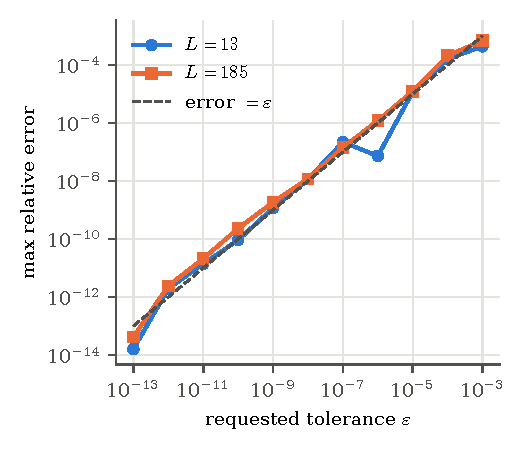
\includegraphics[width=.49\linewidth]{fig/accuracy.pdf}\hfill
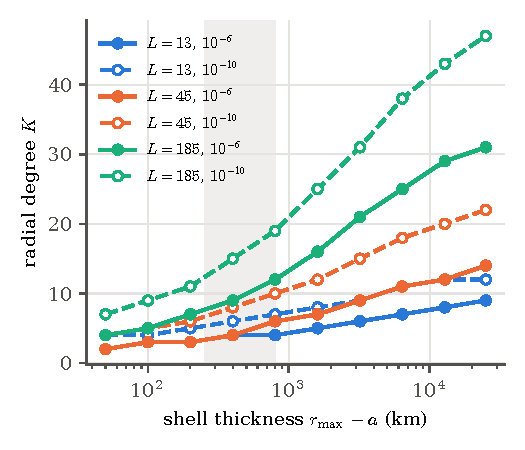
\includegraphics[width=.49\linewidth]{fig/K_thickness.pdf}
\caption{\emph{Left:} achieved maximum relative error over 20\,000 points (including both poles)
versus the requested tolerance $\eps$; the dashed line is error $=\eps$. \emph{Right:} radial
degree $K$ chosen by rule~\eqref{eq:Kchoice} versus shell thickness (inner radius $a$; grey band: the 250--800\,km satellite shell). The
exact value $K=L+2$ is never needed for thin shells.}
\label{fig:acc}\label{fig:K}
\end{figure}

\begin{figure}[!htbp]\centering
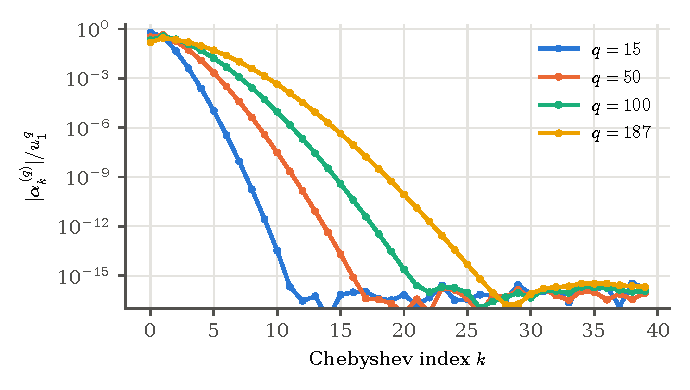
\includegraphics[width=.6\linewidth]{fig/cheb_decay.pdf}
\caption{Magnitude of the Chebyshev coefficients $|\alpha_k^{(q)}|/u_1^q$ of the radial factor $u^q$
on the 250--800\,km shell. The super-geometric decay predicted by~\eqref{eq:bern} means that a
dozen modes reach $10^{-10}$ even for $q=187$.}
\label{fig:cheb}
\end{figure}

\subsection{Speed}

\Cref{fig:speedup} and \cref{tab:speedup} summarise the results. The main findings are:
\begin{itemize}
\item The per-point cost of the transform is essentially independent of $L$
  (\cref{fig:time}). For the direct method it grows as $L^2$.
\item The crossover is at $L\approx15$--$20$ for $\eps=10^{-6}$ and $L\approx25$--$30$ for $\eps=10^{-10}$, as
  predicted by~\eqref{eq:crossover}. \textbf{For the IGRF alone ($L=13$) the direct method is as fast or faster.}
\item At $L=185$ (the full CHAOS static field) and $M=2\times10^6$, the transform is \SPEEDUPDOUBLE\ faster
  at $\eps=10^{-6}$ (\SPEEDUPDOUBLETEN\ at $\eps=10^{-10}$) and \SPEEDUPSINGLE\ faster in single precision.
  It evaluates $2\times10^6$ vector samples in about 2\,s instead of 3.5 minutes.
\item Including the precomputation ($\approx1$\,s at $L=185$), the transform overtakes the direct method at about $2\times10^4$ points
  and is $\approx6\times$ faster at $10^5$ points (\cref{fig:time}).
\item Fixing $\sigma=2$ instead of FINUFFT's automatic choice doubled the high-degree speedups (\cref{tab:upsamp}).
\end{itemize}

\begin{figure}[!htbp]\centering
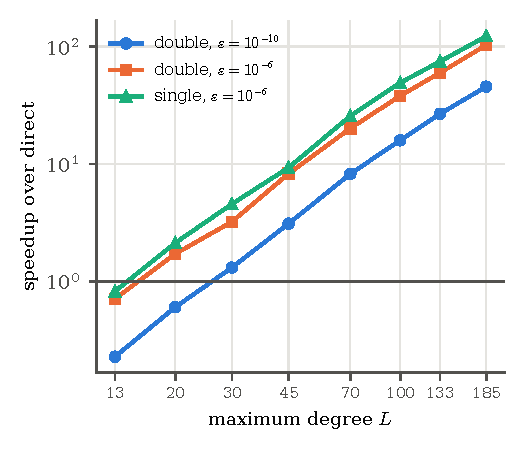
\includegraphics[width=.49\linewidth]{fig/speedup_L.pdf}\hfill
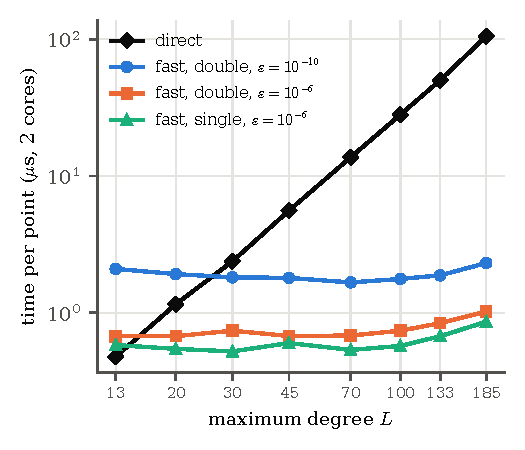
\includegraphics[width=.49\linewidth]{fig/perpoint_L.pdf}
\caption{\emph{Left:} speedup over direct synthesis at $M=2\times10^6$ (evaluation time;
precomputation excluded, see \cref{tab:speedup}). \emph{Right:} time per point. The transform
is flat in $L$, while direct synthesis grows as $L^2$.}
\label{fig:speedup}
\end{figure}

\begin{figure}[!htbp]\centering
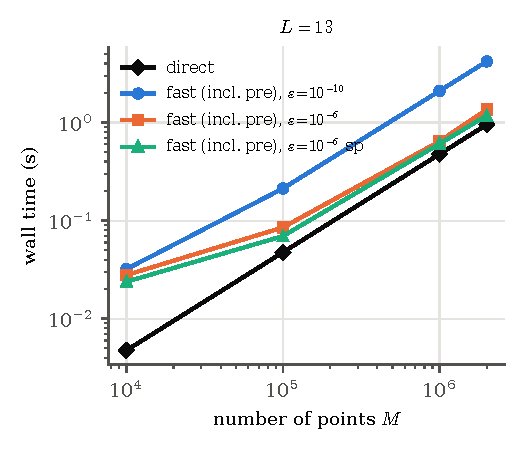
\includegraphics[width=.49\linewidth]{fig/time_M_13.pdf}\hfill
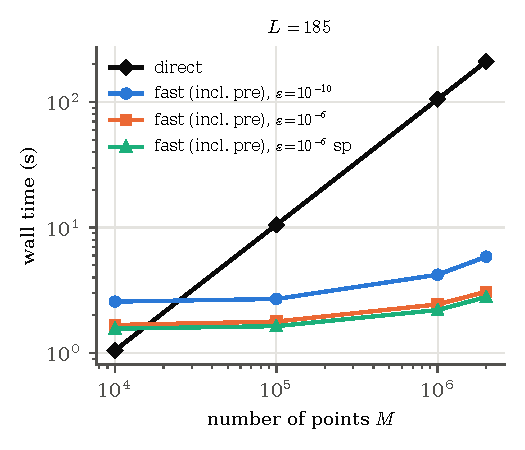
\includegraphics[width=.49\linewidth]{fig/time_M_185.pdf}
\caption{Total wall time (fast transform \emph{including} precomputation) versus number of points, for
$L=13$ (IGRF) and $L=185$ (CHAOS lithosphere).}
\label{fig:time}
\end{figure}

\begin{table}[!htbp]\centering\footnotesize\setlength{\tabcolsep}{3.6pt}
\caption{Benchmark summary (250--800\,km shell, 2 cores). $K$: radial degree chosen automatically. Times for $M=10^6$
points in seconds (fast: evaluation only; precompute listed separately). Speedup is the ratio of evaluation times at
$M=2\times10^6$. The error is the maximum $|\Delta B|$ over the three components versus direct synthesis, in nT
($|\mathbf B|\lesssim 6\times10^4$\,nT). Columns: d10 = double, $\varepsilon=10^{-10}$; d6 = double, $10^{-6}$; s6 = single, $10^{-6}$.}
\label{tab:speedup}
\begin{tabular}{rrrrr@{\hspace{8pt}}rrr@{\hspace{8pt}}rrr@{\hspace{8pt}}rrr}\toprule
&\multicolumn{2}{c}{$K$}&pre&direct&\multicolumn{3}{c}{fast (s)}&\multicolumn{3}{c}{speedup}&\multicolumn{3}{c}{error (nT)}\\
\cmidrule(lr){2-3}\cmidrule(lr){6-8}\cmidrule(lr){9-11}\cmidrule(lr){12-14}
$L$&$10^{-6}$&$10^{-10}$&(s)&(s)&d10&d6&s6&d10&d6&s6&d10&d6&s6\\\midrule
13 & 4 & 6 & 0.008 & 0.48 & 2.09 & 0.63 & 0.59 & 0.2 & 0.7 & 0.8 & 6e-6 & 1e-1 & 1e-1 \\
20 & 4 & 6 & 0.012 & 1.15 & 1.84 & 0.65 & 0.54 & 0.6 & 1.7 & 2.1 & 6e-6 & 9e-2 & 1e-1 \\
30 & 4 & 7 & 0.018 & 2.37 & 1.80 & 0.73 & 0.56 & 1.3 & 3.2 & 4.6 & 6e-6 & 9e-2 & 1e-1 \\
45 & 4 & 8 & 0.041 & 5.58 & 1.80 & 0.70 & 0.59 & 3.1 & 8.3 & 9.3 & 9e-6 & 8e-2 & 2e-1 \\
70 & 5 & 9 & 0.193 & 13.69 & 1.76 & 0.71 & 0.54 & 8.2 & 20.1 & 25.6 & 1e-5 & 8e-2 & 4e-1 \\
100 & 5 & 10 & 0.302 & 28.08 & 1.95 & 0.82 & 0.60 & 15.9 & 38.0 & 49.1 & 7e-6 & 7e-2 & 5e-1 \\
133 & 6 & 11 & 0.588 & 50.19 & 2.02 & 1.01 & 0.80 & 26.8 & 59.9 & 74.6 & 8e-6 & 1e-1 & 7e-1 \\
185 & 6 & 12 & 1.239 & 105.14 & 2.97 & 1.40 & 1.13 & 45.5 & 103.1 & 122.4 & 1e-5 & 6e-2 & 7e-1 \\
\bottomrule\end{tabular}\end{table}

\begin{table}[!htbp]\centering\small
\caption{Breakdown of one evaluation for $M=10^6$ points (3 components, $\sigma=2$, 2 cores). FFT = deconvolution plus FFT
(measured with $10$ points); interpolation = the remainder of the NUFFT time. The interpolation cost per point depends on
$w$ only, not on $L$.}\label{tab:breakdown}
\begin{tabular}{rrrrcrrrr}\toprule
$L$&$\varepsilon$&$w$&$K$&modes $(\psi,\theta,\varphi)$&sort (s)&FFT (s)&interp.\ (s)&$\mu$s/point\\\midrule
13 & $10^{-6}$ & 7 & 4 & $9\times27\times14$ & 0.012 & 0.008 & 0.598 & 0.60\\
13 & $10^{-10}$ & 11 & 6 & $13\times27\times14$ & 0.011 & 0.005 & 1.960 & 1.96\\
185 & $10^{-6}$ & 7 & 6 & $13\times371\times186$ & 0.037 & 0.635 & 0.617 & 0.62\\
185 & $10^{-10}$ & 11 & 12 & $25\times371\times186$ & 0.021 & 1.305 & 1.557 & 1.56\\
\bottomrule\end{tabular}\end{table}

\begin{table}[!htbp]\centering\small
\caption{Effect of the NUFFT oversampling factor on evaluation time ($M=10^6$, seconds). ``auto'' is FINUFFT's heuristic.
$\sigma=1.25$ at $\varepsilon=10^{-10}$ needs a kernel wider than FINUFFT's maximum of 16 points.}\label{tab:upsamp}
\begin{tabular}{rrrrr}\toprule $L$&$\varepsilon$&auto&$\sigma=2$&$\sigma=1.25$\\\midrule
45 & $10^{-6}$ & 0.77 & 0.74 & 1.98\\
45 & $10^{-10}$ & 1.75 & 1.65 & 5.12\\
100 & $10^{-6}$ & 2.03 & 0.95 & 2.02\\
100 & $10^{-10}$ & 1.89 & 1.94 & 5.07\\
185 & $10^{-6}$ & 2.13 & 1.44 & 2.10\\
185 & $10^{-10}$ & 2.87 & 2.75 & 5.12\\
\bottomrule\end{tabular}\end{table}



\subsection{The 2-D variant}\label{sec:results2d}

\Cref{tab:2d} and \cref{fig:2d} compare the fused 2-D variant (\cref{sec:fused}; numba, two threads) with
the 3-D method on the same points.
\begin{itemize}
\item \textbf{Accuracy.} The relative errors against direct synthesis, including both poles, are
  $1.7\times10^{-6}$, $7.2\times10^{-10}$ and $3.7\times10^{-12}$ at $L=13$, and
  $9.2\times10^{-7}$, $5.2\times10^{-10}$ and $3.2\times10^{-12}$ at $L=185$, for $\eps=10^{-6},10^{-10},10^{-12}$.
  The unfused 2-D version, with FINUFFT's kernel, stays within $2.6\eps$.
\item \textbf{Large $M$} ($2\times10^6$). The fused 2-D variant is $1.1$--$2.0\times$ faster than 3-D in 8 of
  10 cases, and 6--11\,\% slower at $\eps=10^{-6}$ for $L=45$ and $L=100$. At $L=185$ it reaches
  $108\times$ ($\eps=10^{-6}$) and $63\times$ ($\eps=10^{-10}$) over direct synthesis, against $94\times$ and $44\times$ for 3-D.
\item \textbf{Moderate $M$} ($10^5$). Without a per-call FFT, the 2-D variant is up to $5.7\times$
  ($\eps=10^{-6}$) and $8.3\times$ ($\eps=10^{-10}$) faster than 3-D at $L=185$.
\item \textbf{Fusion is essential.} Executed as an unfused batch of $3\rho$ FINUFFT transforms, the same
  2-D split runs at only $0.5$--$0.9\times$ the speed of the 3-D method at $M=2\times10^6$.
\item \textbf{IGRF.} At $L=13$, the 2-D variant is still slower than direct synthesis ($0.5$--$0.8\times$).
\end{itemize}
The numba implementation is less optimised than FINUFFT's hand-vectorised code, so the 2-D results are
probably conservative.

\begin{figure}[!htbp]\centering
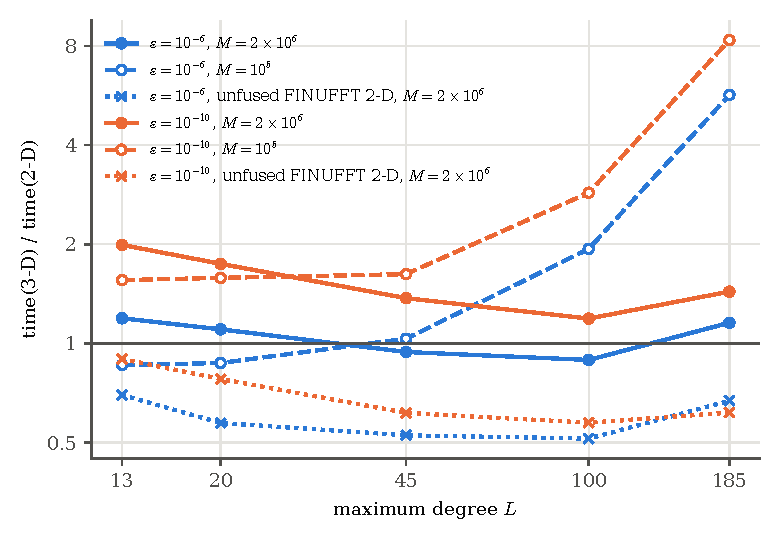
\includegraphics[width=.72\linewidth]{fig/twod_ratio.pdf}
\caption{Speed of the fused 2-D variant relative to the 3-D method (values above 1: 2-D faster), at
$M=2\times10^6$ (solid) and $M=10^5$ (dashed). Crosses: the same 2-D split run as an unfused batch of
FINUFFT transforms.}
\label{fig:2d}
\end{figure}

\begin{table}[!htbp]\centering\footnotesize\setlength{\tabcolsep}{4pt}
\caption{Fused 2-D variant versus the 3-D NUFFT method (FINUFFT), 250--800\,km shell, 2 cores, double precision.
$K+1$: number of Chebyshev radial terms; $\rho$: SVD radial rank (cutoff $0.3\varepsilon$). Times in seconds, evaluation only.
``FINUFFT 2-D'' is the same 2-D split executed as $3\rho$ batched FINUFFT transforms, without fusion.
The last two columns give the speedups over direct synthesis at $M=2\times10^6$.}\label{tab:2d}
\begin{tabular}{rrrr rr rrr r rr}\toprule
&&&&\multicolumn{2}{c}{$M=10^5$}&\multicolumn{3}{c}{$M=2\times10^6$}&3-D/2-D&\multicolumn{2}{c}{vs direct}\\
\cmidrule(lr){5-6}\cmidrule(lr){7-9}\cmidrule(lr){11-12}
$L$&$\varepsilon$&$K{+}1$&$\rho$&3-D&2-D&3-D&2-D&FINUFFT 2-D&($2{\times}10^6$)&3-D&2-D\\\midrule
13 & $10^{-6}$ & 5 & 4 & 0.068 & 0.079 & 1.44 & 1.21 & 2.16 & 1.19 & 0.7 & 0.8\\
13 & $10^{-10}$ & 7 & 6 & 0.243 & 0.156 & 4.20 & 2.11 & 4.72 & 1.99 & 0.2 & 0.5\\
20 & $10^{-6}$ & 5 & 4 & 0.072 & 0.082 & 1.47 & 1.33 & 2.62 & 1.10 & 1.6 & 1.7\\
20 & $10^{-10}$ & 7 & 6 & 0.284 & 0.180 & 4.06 & 2.33 & 4.99 & 1.74 & 0.6 & 1.0\\
45 & $10^{-6}$ & 5 & 4 & 0.123 & 0.119 & 1.48 & 1.57 & 2.57 & 0.94 & 7.5 & 7.1\\
45 & $10^{-10}$ & 9 & 7 & 0.270 & 0.166 & 3.53 & 2.57 & 5.68 & 1.37 & 3.2 & 4.3\\
100 & $10^{-6}$ & 6 & 5 & 0.239 & 0.123 & 1.64 & 1.85 & 3.27 & 0.89 & 34 & 30\\
100 & $10^{-10}$ & 11 & 8 & 0.526 & 0.184 & 3.60 & 3.03 & 6.29 & 1.19 & 16 & 19\\
185 & $10^{-6}$ & 7 & 5 & 0.772 & 0.136 & 2.24 & 1.94 & 3.38 & 1.15 & 94 & 108\\
185 & $10^{-10}$ & 13 & 9 & 1.639 & 0.197 & 4.80 & 3.35 & 7.68 & 1.44 & 44 & 63\\
\bottomrule\end{tabular}\end{table}



\subsection{Machine precision}\label{sec:results-exact}

To measure the true error, we computed a reference in x87 long-double arithmetic (64-bit mantissa, about 19
significant digits) with the same recursions, at 1500 points including both poles. Against this reference, the
direct double-precision sum has a relative error of $1.1\times10^{-15}$ at $L=13$ and $1.6\times10^{-14}$ at $L=185$
($9\times10^{-10}$\,nT), caused by rounding in the recursions. This is the floor any double-precision method must reach
to count as exact.

\Cref{tab:wscan} shows how the error of the fused 2-D transform falls with the kernel width. It reaches the direct
sum's floor at $w=16$ ($\sigma=2$), $w=13$ ($\sigma=3$) or $w=12$ ($\sigma=4$). Larger oversampling allows a narrower
kernel, at the cost of a larger stored grid. \Cref{tab:exact} gives the timings at this accuracy. With $\sigma=3$ and
$w=13$, the 2-D transform is \emph{as accurate as the direct sum} and still $42\times$ faster at $L=185$, $13\times$ at
$L=100$ and $3\times$ at $L=45$. At degree 13--20 it is slower than the direct sum.

\begin{table}[!htbp]\centering\footnotesize\setlength{\tabcolsep}{3pt}
\caption{Maximum relative error of the fused 2-D transform against a 19-digit (long double) reference, as a function of
kernel width $w$ and oversampling $\sigma$ ($L=185$, 1500 points including both poles, radial rank $\rho=14$).
For comparison, the direct double-precision sum has error $1.6\times10^{-14}$. Grid sizes are the stored oversampled grids.}\label{tab:wscan}
\begin{tabular}{lccccccccc}\toprule
&$w=8$ & $w=9$ & $w=10$ & $w=11$ & $w=12$ & $w=13$ & $w=14$ & $w=15$ & $w=16$\\\midrule
$\sigma=2$ (190\,MB) & $2\times10^{-7}$ & $1\times10^{-8}$ & $4\times10^{-9}$ & $6\times10^{-10}$ & $6\times10^{-11}$ & $3\times10^{-12}$ & $3\times10^{-13}$ & $7\times10^{-14}$ & $2\times10^{-14}$\\
$\sigma=3$ (421\,MB) & $2\times10^{-8}$ & $2\times10^{-9}$ & $2\times10^{-10}$ & $2\times10^{-11}$ & $1\times10^{-12}$ & $3\times10^{-14}$ & -- & -- & --\\
$\sigma=4$ (749\,MB) & $6\times10^{-9}$ & $8\times10^{-10}$ & $6\times10^{-11}$ & $4\times10^{-12}$ & $7\times10^{-14}$ & $3\times10^{-14}$ & -- & -- & --\\
\bottomrule\end{tabular}\end{table}

\begin{table}[!htbp]\centering\small\setlength{\tabcolsep}{4.5pt}
\caption{Fused 2-D transform at machine precision versus direct synthesis, $M=10^6$ points, 250--800\,km shell, 2 cores.
``Machine precision'' means a relative error of $\approx2$--$3\times10^{-14}$ against a long-double reference, the same as
the direct double-precision sum (\cref{tab:wscan}). $\rho$: radial rank (tolerance $10^{-15}$). Times in seconds, evaluation only.}\label{tab:exact}
\begin{tabular}{rrr rr rrr rr}\toprule
&&&\multicolumn{2}{c}{$\sigma=2$, $w=16$}&\multicolumn{3}{c}{$\sigma=3$, $w=13$}&\multicolumn{2}{c}{$\varepsilon\approx10^{-10}$, $w=12$}\\
\cmidrule(lr){4-5}\cmidrule(lr){6-8}\cmidrule(lr){9-10}
$L$&$\rho$&direct&time&speedup&time&speedup&grid (MB)&time&speedup\\\midrule
13 & 8 & 0.48 & 2.24 & 0.2 & 1.58 & 0.3 & 1 & 1.31 & 0.4\\
20 & 9 & 1.15 & 2.37 & 0.5 & 1.67 & 0.7 & 3 & 1.32 & 0.9\\
45 & 10 & 5.58 & 2.43 & 2.3 & 1.88 & 3.0 & 19 & 1.62 & 3.5\\
100 & 12 & 28.08 & 3.19 & 8.8 & 2.20 & 13 & 108 & 1.60 & 18\\
185 & 14 & 105.14 & 3.30 & 32 & 2.48 & 42 & 421 & 1.83 & 58\\
\bottomrule\end{tabular}\end{table}


%=====================================================================
\section{Recommendations and limitations}\label{sec:limits}
%=====================================================================
\begin{itemize}
\item \textbf{When to use it.} Use the transform for models with $L\gtrsim20$ (at $\eps\approx10^{-6}$) or
  $L\gtrsim30$ (at $\eps\approx10^{-10}$) and more than about $10^5$ points, i.e.\ lithospheric and
  high-resolution core models. For IGRF alone, a well-written direct evaluator is already near-optimal.
\item \textbf{2-D or 3-D.} With a fused implementation, the 2-D variant (\cref{sec:2d}) is the faster choice
  on satellite shells, especially for $M\lesssim10^6$ at high $L$, where it avoids the per-call FFT. Prefer the 3-D method
  for wide radial ranges where $\rho>w$ (or split the range into shells), or when only an off-the-shelf NUFFT library is used.
  Do not run the 2-D split as an unfused batch of library transforms: that is slower than 3-D.
\item \textbf{Exact results.} For results indistinguishable from the direct double-precision sum, use the fused 2-D
  transform with $\sigma=3$, $w=13$ and radial tolerance $10^{-15}$ (\cref{tab:exact}).
\item \textbf{Accuracy setting.} $\eps=10^{-6}$ to $10^{-7}$ relative already corresponds to about 0.05\,nT,
  well below data noise and model uncertainty, and is about twice as fast as $10^{-10}$.
  Single precision is another $1.3$--$2\times$ faster, with $\approx10^{-5}$ relative accuracy at high $L$.
\item \textbf{Time dependence} multiplies the interpolation cost by the number of active
  coefficient sets $J$. Use the hybrid strategy for CHAOS (\cref{sec:extensions}).
\item \textbf{Memory.} The tensor and the oversampled NUFFT grid scale as $KL^2$. For very wide radial ranges at
  high $L$, split the range into shells.
\item \textbf{Range.} The transform is valid only inside $[r_{\min},r_{\max}]$ (points outside are rejected).
\end{itemize}

%=====================================================================
\section{Reference implementation}\label{sec:impl}
%=====================================================================
The package \texttt{fastpot} (Python; dependencies \texttt{numpy}, \texttt{finufft}, \texttt{numba}) contains:
\begin{itemize}
\item \texttt{fastpot.py}: the 3-D transform, \texttt{FastInternalField};
\item \texttt{fastpot.py}: the unfused 2-D split, \texttt{FastInternalField2D} (SVD or Chebyshev radial
  basis, batched FINUFFT transforms);
\item \texttt{fused2d.py}: the fused 2-D variant with cached grids (\texttt{FusedField2D});
\item \texttt{direct.py}: the direct baseline;
\item \texttt{test\_validate.py} and \texttt{test\_time.py}: validation against \texttt{ppigrf};
\item the benchmarks reported here: \texttt{bench.py}, \texttt{experiments.py}, \texttt{bench2d.py},
  \texttt{bench\_fused.py} and \texttt{bench\_exact.py};
\item \texttt{refld.py}: the long-double reference used in \cref{sec:results-exact}.
\end{itemize}
Usage:
\begin{lstlisting}
from fastpot import FastInternalField
T = FastInternalField(g, h, a=6371.2, rmin=6371.2+250, rmax=6371.2+800, eps=1e-8)
Br, Btheta, Bphi = T(r_km, theta_rad, phi_rad)        # B_N=-Btheta, B_E=Bphi, B_C=-Br
# time-dependent: g,h of shape (J,L+1,L+1); weights W of shape (M,J)
Br, Btheta, Bphi = T_td(r_km, theta_rad, phi_rad, weights=W)
# 2-D variant (fused, cached grids; single coefficient set)
from fused2d import FusedField2D
F = FusedField2D(g, h, a=6371.2, rmin=6371.2+250, rmax=6371.2+800, eps=1e-8)
Br, Btheta, Bphi = F(r_km, theta_rad, phi_rad)
# machine precision: kernel width w, oversampling sigma, radial SVD tolerance
F = FusedField2D(g, h, rmin=6371.2+250, rmax=6371.2+800, w=13, sigma=3.0, eps_radial=1e-15)
\end{lstlisting}
The core of the precomputation (one order $m$) and of the evaluation is:
\begin{lstlisting}
for m in range(L + 1):
    P, dP, Q = legendre_column(m, ...)            # n = m..L on theta grid (doubled sphere)
    Ph, dPh, Qh = fft_theta(P), fft_theta(dP), fft_theta(Q)   # exact modes |p| <= L
    c  = g[n, m] - 1j*h[n, m]
    Rn = R[:, n + 2]                              # radial Chebyshev modes of u^(n+2)
    F[0, :, :, m] = Rn @ (((n + 1) * c)[:, None] * Ph)        # B_r
    F[1, :, :, m] = Rn @ ((-c)[:, None] * dPh)                # B_theta
    F[2, :, :, m] = Rn @ ((-1j * m * c)[:, None] * Qh)        # B_phi
# evaluation
psi = arccos((a/r - uc)/ud)
plan.setpts(psi, theta, wrap(phi));  out = plan.execute(F)   # one batched 3-D NUFFT
B = real(out * exp(1j*m0*phi))
\end{lstlisting}

%=====================================================================
\appendix
\section{Pole-safe recursions}\label{app:recursions}
%=====================================================================
Let $x=\cos\theta$ and $s=\sin\theta$, where $s$ is \emph{signed} on the doubled sphere. Write $Q_n^m=P_n^m/s$ for $m\ge1$.

\paragraph{Sectoral seeds.} $P_0^0=1$, $\mathrm dP_0^0=0$; $P_1^1=s$, $\mathrm dP_1^1=x$, $Q_1^1=1$. For $m\ge2$, with $f_m=\sqrt{(2m-1)/(2m)}$:
\[
P_m^m=f_m\,s\,P_{m-1}^{m-1},\qquad
\mathrm dP_m^m=f_m\big(s\,\mathrm dP_{m-1}^{m-1}+x\,P_{m-1}^{m-1}\big),\qquad
Q_m^m=f_m\,s\,Q_{m-1}^{m-1}.
\]
\paragraph{Upward in $n$.} With $A_n^m=\frac{2n-1}{\sqrt{n^2-m^2}}$ and $B_n^m=\sqrt{\frac{(n-1)^2-m^2}{n^2-m^2}}$ (and $B=0$ for $n=m+1$):
\begin{align*}
P_n^m&=A_n^m\,x\,P_{n-1}^m-B_n^mP_{n-2}^m,\\
\mathrm dP_n^m&=A_n^m\big(x\,\mathrm dP_{n-1}^m-s\,P_{n-1}^m\big)-B_n^m\,\mathrm dP_{n-2}^m,\\
Q_n^m&=A_n^m\,x\,Q_{n-1}^m-B_n^mQ_{n-2}^m.
\end{align*}
The recursion for $Q$ is the same as the one for $P$, applied to the seed $Q_m^m=P_m^m/s$, which is available in closed
form. No step divides by $\sin\theta$, so all quantities are exact trigonometric polynomials
evaluated stably at every $\theta$, including the poles.

\section{Chebyshev modes of \texorpdfstring{$u^q$}{u^q} by interpolation}
With $\psi_j=\pi j/K$, $u_j=u_c+u_d\cos\psi_j$ and $f_j=u_j^q$, $j=0..K$:
\[
\alpha_k=\frac{2}{K}\,{\sum_{j=0}^{K}}{}''\,f_j\cos\frac{\pi jk}{K},\qquad
\alpha_0,\alpha_K\ \text{halved},
\]
where $\sum''$ halves the first and last terms. For $K\ge q$ these are exactly the coefficients of
\cref{lem:radial}; for $K<q$ they define the Chebyshev interpolant, whose error is at most twice the tail.

\begin{thebibliography}{99}\small
\bibitem{alken2021} P.~Alken et al., International Geomagnetic Reference Field: the thirteenth generation, \emph{Earth, Planets and Space} 73:49 (2021).
\bibitem{finlay2020} C.~C.~Finlay, C.~Kloss, N.~Olsen, M.~D.~Hammer, L.~T\o ffner-Clausen, A.~Grayver, A.~Kuvshinov, The CHAOS-7 geomagnetic field model and observed changes in the South Atlantic Anomaly, \emph{Earth, Planets and Space} 72:156 (2020).
\bibitem{dutt1993} A.~Dutt, V.~Rokhlin, Fast Fourier transforms for nonequispaced data, \emph{SIAM J.\ Sci.\ Comput.} 14(6):1368--1393 (1993).
\bibitem{greengard2004} L.~Greengard, J.-Y.~Lee, Accelerating the nonuniform fast Fourier transform, \emph{SIAM Review} 46(3):443--454 (2004).
\bibitem{barnett2019} A.~H.~Barnett, J.~Magland, L.~af~Klinteberg, A parallel nonuniform fast Fourier transform library based on an ``exponential of semicircle'' kernel, \emph{SIAM J.\ Sci.\ Comput.} 41(5):C479--C504 (2019).
\bibitem{kunis2003} S.~Kunis, D.~Potts, Fast spherical Fourier algorithms, \emph{J.\ Comput.\ Appl.\ Math.} 161:75--98 (2003).
\bibitem{keiner2009} J.~Keiner, S.~Kunis, D.~Potts, Using NFFT 3 --- a software library for various nonequispaced fast Fourier transforms, \emph{ACM Trans.\ Math.\ Softw.} 36(4), Art.~19 (2009).
\bibitem{driscoll1994} J.~R.~Driscoll, D.~M.~Healy, Computing Fourier transforms and convolutions on the 2-sphere, \emph{Adv.\ Appl.\ Math.} 15:202--250 (1994).
\bibitem{schaeffer2013} N.~Schaeffer, Efficient spherical harmonic transforms aimed at pseudospectral numerical simulations, \emph{Geochem.\ Geophys.\ Geosyst.} 14(3):751--758 (2013).
\bibitem{borodin1974} A.~Borodin, R.~Moenck, Fast modular transforms, \emph{J.\ Comput.\ Syst.\ Sci.} 8:366--386 (1974).
\bibitem{slepian1961} D.~Slepian, H.~O.~Pollak, Prolate spheroidal wave functions, Fourier analysis and uncertainty~I, \emph{Bell Syst.\ Tech.\ J.} 40:43--63 (1961).
\bibitem{anderson1996} C.~Anderson, M.~D.~Dahleh, Rapid computation of the discrete Fourier transform, \emph{SIAM J.\ Sci.\ Comput.} 17(4):913--919 (1996).
\bibitem{ruiz2018} D.~Ruiz-Antol\'in, A.~Townsend, A nonuniform fast Fourier transform based on low rank approximation, \emph{SIAM J.\ Sci.\ Comput.} 40(1):A529--A547 (2018).
\bibitem{trefethen2013} L.~N.~Trefethen, \emph{Approximation Theory and Approximation Practice}, SIAM (2013).
\end{thebibliography}

\end{document}
